\documentclass[a4j,9pt,twocolumn]{jsarticle}

%\usepackage{multicol} %2段組み用
\usepackage{amsmath}  %alignなど数式関係で必要になることが多い.
%\usepackage{graphicx} %図の取り込みに利用.
\usepackage[dvipdfmx]{graphicx} %図の取り込みに利用.
\usepackage{url}      %URLの表記に使う\urlコマンドに必要.
\usepackage{txfonts}  %英文をTimes Romanのようなフォントにする.
                      %通常のLaTeXのフォントにしたいときはこれをコメントアウトする.
\usepackage{algorithm,algorithmic} %algorithmとalgorithmic環境を利用するのに必要.
\usepackage{enumerate}%enumerate環境で項目を[Step 1.]のような形式に変更するのに利用.
\usepackage{ascmac} %itembox環境を利用するのに必要
\usepackage{longtable} 
\usepackage{multicol} % 複数列の箇条書き

\pagestyle{plain} %ページ番号のスタイル
\urlstyle{same}   %\urlコマンドのフォント指定."tt", "rm", "sf", "same"(=使用中のフォント)

%%%%%%%%%%%%%%%%%%%%%%%%%%%%%% ↓テキスト幅,マージン,行間の調節
\textwidth     =  195mm %テキスト幅
\oddsidemargin = -7.5mm %左側のマージン
\textheight    =  280mm %テキストの高さ
\topmargin     =  -10mm %上のマージン
\renewcommand{\baselinestretch}{0.85} %行間を調節
%%%%%%%%%%%%%%%%%%%%%%%%%%%%%% ↑テキスト幅,マージン,行間の調節

%%%% ↓Change the style of itemize, enumerate, etc.
%%%% ↓(without space between items)
\makeatletter
\def\@listI{\leftmargin\leftmargini
    \topsep  \z@
    \parsep  \z@
    \itemsep \z@}
\let\@listi\@listI
\@listi 
\def\@listii{\leftmargin\leftmarginii
    \labelwidth\leftmarginii\advance\labelwidth-\labelsep
    \topsep  \z@
    \parsep  \z@
    \itemsep \z@}
\def\@listiii{\leftmargin\leftmarginiii
    \labelwidth\leftmarginiii\advance\labelwidth-\labelsep
    \topsep  \z@
    \parsep  \z@
    \itemsep \z@}
\makeatother
%%%% ↑Change the style of itemize, enumerate, etc.

%%%% ↓algotithmic の \REQUIRE と \ENSURE の表記を変更する
\renewcommand{\algorithmicrequire}{\textbf{Input:}}
\renewcommand{\algorithmicensure}{\textbf{Output:}}
%%%% ↑algotithmic の \REQUIRE と \ENSURE の表記を変更する

\newcommand\coleq{\mathrel{\mathop:}=}% \coleqの定義(:=をきれいに出力する)

\begin{document}
\pagestyle{empty} % ページ番号を表示しない.
\twocolumn[%
\begin{center}
 {\Large \textbf{セキュアなV2Vアドホックネットワークルーティング\\
 プロトコルのためのEdDSA署名方式の評価}}\\
 \vspace{2mm}
 {\large 工学部 電気電子・情報工学科 情報コース 三嶋研究室 永野正剛 } \\
\end{center}
\vspace{5mm}
]

\section{はじめに}
\textbf{VANET (Vehicle Ad hoc Network)}とは, 移動する車両間で通信を行うための
モバイルアドホックネットワークである. VANETの実用化には高い通信性能とセキュリティの
確保の両立が求められるため, セキュリティの確保に伴う処理の効率化が重要である. 
階戸が提案したデジタル署名を用いたセキュアなV2Vアドホックネットワークルーティング
プロトコル\cite{shinato}は, セキュリティの確保を達成しているが, さらなる処理効率の
向上が求められる. そこで本研究では, 階戸が提案したルーティングプロトコルにおいて, 
比較的新しい署名方式であるEdDSA (Edwards-curve Digital Signature Algorithm)を採用し, 
セキュリティ確保に伴う処理の効率化を図った.  
その性能を階戸の研究と比較して評価するため, 離散型ネットワークシミュレータ ns-3用いて, 
ネットワークへの負荷や同一エリア内のノード数に対する拡張性を調査するシミュレーション実験を
行った. 
\section{関連技術, 関連研究}
\noindent \textbf{(1) GPSR}\\
\indent \textbf{GPSR (Greedy Perimeter Stateless Routing)}\cite{gpsr}は, ノードの位置情報と
IPアドレスを用いるルーティングプロトコルである. 各ノードは, 以下の処理を行い, 
ルーティングを構築する. 
\begin{itembox}[l]{GPSRの処理}
  \begin{itemize}
    \item 自身の位置情報とIPアドレスを載せたHelloパケットを一定間隔で
    ブロードキャストする.
    \item 受信したHelloパケットの情報を用いて隣接ノードテーブルを更新する.
  \end{itemize}
\end{itembox}

\noindent\textbf{(2) EdDSA}\\
\indent \textbf{EdDSA}は,  2011年にDaniel J. Bernsteinらによって提案され, 
近年, 標準化された比較的新しいデジタル署名方式である\cite{eddsa}. EdDSAは階戸の研究で
使用されたECDSAに比べて演算が高速で, シンプルかつ堅牢な設計をもつ. 
EdDSAの最も一般的な実装に\textbf{Ed25519}があり, 計算効率とセキュリティのバランスが
取れた性能となっている. 以下にECDSAと比較したEdDSAの特徴を, セキュリティと
処理時間の観点から示す.\\
\noindent \textbf{セキュリティ}\\
(i) 決定論的な署名生成\\
\indent EdDSAは, メッセージと秘密鍵をハッシュすることで署名生成に使用するランダムな
数値を決定論的に生成し, 乱数生成の失敗による秘密鍵の漏洩リスクを回避している.\\
\noindent{\textbf{処理時間}}\\
(i) 乱数生成の回避 \\
\indent 一般的に, 暗号的に安全な乱数は生成の時間がランダムで処理コストが高い. 
EdDSAでは乱数を鍵生成でのみ使用しており, 署名生成, 署名検証では
乱数を使用せず, それらを一定時間で行うため, 乱数を使用するアルゴリズムに比べて
高速に処理することができる.\\
(ii) 乗法逆元の不要\\
\indent EdDSA (Ed25519)では拡張した射影座標系(拡張ツイストエドワーズ座標)で
計算することがRFC8032で推奨されている\cite{8032}. 
この座標系の特性により, 処理コストの高いスカラー値の乗法逆元の処理が不要となる. 
したがって, 処理が単純化され,  高速化しやすい.\\[2mm]
\noindent\textbf{(3) 階戸のプロトコル}\\
\indent GPSRでは, 同一アドホックネットワークの参加者が相互に正しい位置情報を
送信しない限り, ルーティングが正しく行われない. そのため, 階戸のプロトコルではノード情報に
デジタル署名を付与することで, なりすましや改ざんを排除している. 具体的には, 送信者が
ノード情報(IPアドレス, 位置情報)の正当性を担保する認証機関からの署名をHelloパケットに
付加して送信し, 受信者はそれらの署名の検証に成功した場合のみノードテーブルを
更新する(図\ref{fig:introduce}). 
署名者(認証機構)と被署名データの対応を表\ref{tab:sign}に示す. 
\vspace{-3mm}
\begin{table}[h]
    \centering
    \caption{署名者と被署名データの対応\cite{shinato}}
    \label{tab:sign}
    \begin{tabular}{cc} \hline
        署名者 & 被署名データ \\ \hline \hline
        DHCPサーバ & IPアドレス \\
        位置情報認証機関 & 位置情報 \\ \hline
    \end{tabular}
\end{table}
\vspace{-5mm} % ← ここで表と図の間の余白を詰める
\begin{figure}[h]
    \centering
    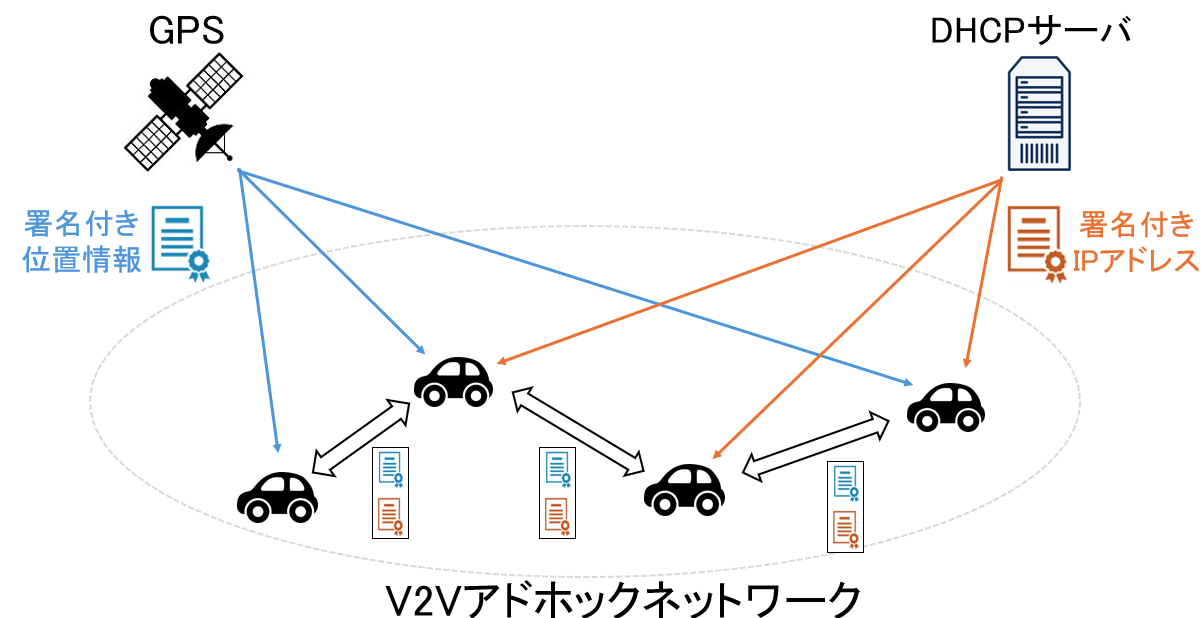
\includegraphics[width=0.45\textwidth]{figures/introduce.png}
    \caption{階戸のプロトコル\cite{shinato}}
    \label{fig:introduce}
\end{figure}
\vspace{-5mm}
\section{提案手法}
\indent EdDSAの処理効率の高さが階戸のプロトコルに及ぼす影響を調査し, EdDSAの実装を
評価するために, 以下の手順を踏んだ. 
\noindent\textbf{(1) EdDSAの導入}\\
\indent EdDSAの最も一般的な実装であるEd25519を階戸のプロトコルに導入し, 
階戸と同様のシミュレーション環境でシミュレーション実験を行う. 
階戸の研究では, ns-3のGPSRモジュールにOpen SSLのDSAとECDSAの署名機能を追加する
コーディングしていた. 本研究では, EdDSAを導入するために, Open SSLのEd25519の署名機能を
GPSRモジュールに追加するコーディングを行った. \\
\noindent\textbf{(2) 評価基準の選定}\\
\indent EdDSAの性能を評価をするために, 以下の評価基準を用いる. 
\vspace{-3mm}
\begin{multicols}{2}
    \begin{enumerate}
        \item スループット
        \item 遅延時間 (Delay)
        \item パケット配送率 (PDR)
        \item オーバーヘッドサイズ\\
        \item シミュレーション実行時間
        \item 署名作成時間
        \item 署名検証時間
        \item メモリ使用量
    \end{enumerate}
\end{multicols}
\vspace{-3mm}
これらをシミュレーション結果として採取し, 署名方式の違いによる性能差を評価する. 

\section{シミュレーション実験}
本研究では, ns-3を用いて3つのシミュレーション実験を行った. 主要な
シミュレーションパラメータを表\ref{tab:parameter}に示す. 
\begin{table}[h]
  \centering
  \caption{シミュレーションパラメータ}
  \label{tab:parameter}
  \begin{tabular}{ll} \hline
    シミュレーションツール & ns-3.26 \\
    通信規格 & IEEE 802.11p \\
    通信プロトコル & UDP \\
    パケットサイズ & 1024 [byte] \\
    パケット送信間隔 & 1.0 [s] \\
    送信電力 & 17.026 [dBm] \\
    電力検出閾値 & -96.0 [dBm] \\
    電波伝搬減衰モデル & 対数距離電波伝搬減衰モデル \\
    遅延モデル & 定常速度伝搬モデル \\
    電波伝搬範囲 & 約300 [m] \\
    ノード数 & 74 (実験1, 2)\\
    & 37/74/112/148/185 (実験3) \\
    シミュレーション時間 & 300 [s] \\
    ルーティングプロトコル & GPSR \\
    デジタル署名 & DSA, ECDSA, EdDSA \\ \hline
  \end{tabular}
\end{table}

\indent いずれの実験でも, 以下の4パターンを調べた. 
\begin{itemize}
    \item 認証機構を用いない場合
    \item DSAを用いて認証機構を追加した場合
    \item ECDSAを用いて認証機構を追加した場合
    \item EdDSAを用いて認証機構を追加した場合
\end{itemize}

\subsection{実験1}
実験1では, 認証機構が正しく機能していることを確認するための実験を行った. 
全ノード約8\%を不正ノードを設定し, 250回シミュレーションを行った. 
導入する不正ノードは以下の2種類である. 
\begin{enumerate}
    \item 位置情報を詐称するノード (4\%)\\
    \indent  通信データの窃取を目的に, 偽装した位置情報をHelloパケットで送信する不正ノード. 
    \item IPアドレスを詐称するノード (4\%)\\
    \indent  不正アクセスを目的に, 偽装したIPアドレスをHelloパケットで送信する不正ノード. 
\end{enumerate}
実験1の結果を以下に示す.
\begin{table}[h]
    \centering
    \caption{実験1のシミュレーション結果}
    \label{tab:exp1} 
    \begin{tabular}{l|crrr} \hline
        評価基準 & 認証無し & DSA & ECDSA & EdDSA \\ \hline \hline
        PDR[\%] & $48.2$ & $88.15$ & $86.62$ & $84.48$ \\
        Throughput[kbps] & $4.18$ & $7.64$ & $7.51$ & $7.33$ \\ \hline
    \end{tabular}
\end{table}

表\ref{tab:exp1}は, シミュレーションパターンごとのパケット配送率とスループットを示している. 
認証機構を追加したプロトコルは, パケット配送率とスループットが同程度向上した. 
しかし, 署名方式の違いによる差異はないため, 3つの署名方式が同等の性能をもつと考えられる. 

\subsection{実験2}
\indent 実験2では, 認証機構の追加が通信にどれだけの負荷を与えるのかを調査するための実験を
行った. 不正ノードの存在しない環境で, 250回シミュレーションを行った. \\
\indent 実験2の結果を以下に示す. 
\vspace{-3mm}
\begin{table}[h]
    \centering
    \caption{実験2のシミュレーション結果}
    \label{tab:exp2} 
    \begin{tabular}{l|rrrr} \hline
        評価基準 & 認証無し & DSA & ECDSA & EdDSA \\ \hline \hline
        \footnotesize{median of Delay[ms]} & $6.88$ & $6.13$ & $6.20$ & $84.48$ \\
        \small{mode of Delay[ms]} & $[6.0, 7.0)$ & $[2.0, 3.0)$ & $[2.0, 3.0)$ & $[6.0, 7.0)$ \\
        PDR[\%] & $83.21$ & $87.80$ & $86.89$ & $87.39$ \\
        Overhead[KB] & $2694.3$ & $5982.8$ & $5384.2$ & $5364.5$ \\ \hline
    \end{tabular}
\end{table}

表\ref{tab:exp2}は, シミュレーションパターンごとの遅延時間の中央値と最頻値, 
パケット配送率, オーバーヘッドを示している. この結果は, 遅延時間は経路選択の
タイミングによって左右されるため, 若干の差異が出てしまうが, 認証機構の有無が遅延時間に
影響を与えなかったことを示唆している. また, 認証機構の有無はパケット配送率に影響を
与えなかったことがわかる. オーバーヘッドサイズは, 認証機構を追加することで,
大幅に増加した. これは, Helloパケットのデータに署名が付与されていることが原因である. 
また, 署名方式の違いによる差は, 各署名方式で用いられる鍵長の長さが原因であると考えられる. 
なお, 本研究で使用したパラメータによるそれぞれの鍵長は, DSAで2048ビット, ECDSAとEdDSAで
256ビットである. 

\subsection{実験3}
\indent 実験3では, 同一エリア内のノード数に対する拡張性を調査するための実験を行った. 
不正ノードの存在しない環境でノード数を37, 74, 112, 148, 185に設定し, それぞれ250回ずつ
シミュレーションを行った. \\
\indent 実験3の結果を以下に示す. 
\begin{table}[h]
    \centering
    \caption{ノード数によるシミュレーション実行時間}
    \label{tab:exp3_simtime}
    \begin{tabular}{c|rrrr} \hline
        Number of nodes & \multicolumn{4}{c}{シミュレーション実行時間 [s]} \\ \cline{2-5}
                       & No Auth. & DSA & ECDSA & EdDSA \\ \hline \hline
        37  &  14.18  &   69.99  &   55.01  &   24.41  \\
        74  &  50.60  &  267.43  &  194.41  &   89.27  \\
        112 & 110.41  &  625.50  &  436.93  &  200.90  \\
        148 & 196.97  & 1172.57  &  910.37  &  431.35  \\
        185 & 345.06  & 1908.70  & 1324.55  &  635.16  \\ \hline
    \end{tabular}
\end{table}
\vspace{-5mm}
\begin{table}[h]
    \centering
    \caption{実験3のシミュレーション結果}
    \label{tab:exp3_sig} 
    \begin{tabular}{c|crr} \hline
        評価基準 & 認証無し & ECDSA & EdDSA \\ \hline \hline
        署名生成時間[ms] & 署名無し & $0.371$ & $0.031$ \\
        署名検証時間[ms] & 署名無し & $0.336$ & $0.097$ \\
        メモリ使用量[KB] & $73742.9$ & $151699.0$ & $106226.0$ \\ \hline
    \end{tabular}
\end{table}

表\ref{tab:exp3_simtime}は, シミュレーションパターンごとのノード数による実行時間の変化を, 
表\ref{tab:exp3_sig}はECDSAとEdDSAが1回の署名作成と署名検証にかかった時間と, 
ノード数74の場合のメモリの使用量を示したものである. \\
\indent ECDSAとEdDSAに注目して結果を評価すると, EdDSAの方が実行時間, 署名の生成と
検証の時間が短く, メモリ使用量も小さかった. これらの結果は, EdDSAがECDSAよ
りもスケーラビリティに優れていることを示唆している. 

\section{まとめ}
\indent 実験結果の評価から, EdDSAはECDSAよりも計算効率が高いことがわかった. 
これは, EdDSAの設計上の特長である高速な処理能力が実験環境においても十分に発揮されたことを
示している. また, EdDSAはそのセキュリティの堅牢さから, 秘密鍵を特定しようとする攻撃者が
存在する環境でECDSAよりも高いセキュリティを提供できる. したがって, 階戸のプロトコルにおいて, 
EdDSAはECDSAよりも安全かつ効率的な認証方式として利用できるといえる. 



\noindent\hrulefill % 参考文献の上に線を引く
%%%%%%%%%%%%%%%%%%%%%%%%%%%%%%%%%%%%%%%%%%%%%%%%%%%%%%%%%%%% References
\begin{thebibliography}{99}
    \bibitem{shinato} 階戸 弾,
        \textit{デジタル署名を用いたセキュアなV2Vアドホックルーティングプロトコル},
        Master's thesis, University of Gifu, 2024.
    \bibitem{8032} Simon Josefsson and Ilari Liusvaara, 
        RFC 8032: Edwards-Curve Digital Signature Algorithm (EdDSA), 2017.
    \bibitem{gpsr} Brad Karp and H. T. Kung, 
        \textit{GPSR: Greedy Perimeter Stateless Routing for Wireless Networks},
        Proceedings of the 6th annual international conference on Mobile computing and networking, 2000.
    \bibitem{eddsa} Daniel J. Bernstein, Niels Duif, Tanja Lange, Peter Schwabe, and Bo-Yin Yang,
        \textit{High-speed high-security signatures}, Journal of Cryptographic Engineering, 2011.
\end{thebibliography}

%%%%%%%%%%%%%%%%%%%%%%%%%%%%%%%%%%%%%%%%%%%%%%%%%%%%%%%%%%%%
\end{document}











% 必要な情報を
% 順序よく(つまり後ろを見ないと分からないことが出て来たりしないように),
% 明確に(曖昧さなく厳密に),
% コンパクトに(冗長な表現を無くして手短に)書くよう心がけましょう.
% 構成は研究テーマや書きたいことによって様々ですが,
% 例えばある問題に対するアルゴリズムを提案して,
% その効果を計算実験によって検証するようなテーマであれば,はじめにの節ののち,
% 問題の説明,提案手法の説明,計算実験の紹介,まとめという構成がしばしば用いられます.
% 以下の節ではそのような説明を書く際によく利用する書式や書くべきことの例をいくつか示しておきます.



% \section{実験結果}
% 実験結果を示す際には,計算環境(実験に用いた計算機のCPUやメモリー,
% 実装に用いた言語)を明記しましょう.
% 計算結果を表示するのに用いる図や表を表示する例を図\ref{fig1}と
% 表\ref{table1}に示しておきます.
% また,2段組みの原稿において幅の広い表を表示する例を\mbox{表\ref{table2}}に示しておきます
% (図も同様に\verb#\begin{figure*}#のようにすればよい).


% \begin{table}[htbp]
%  \centering
%  \tabcolsep = 15pt
%  \renewcommand{\arraystretch}{0.8}
%  \caption{表の表示例}
%  \label{table1}
%  \begin{tabular}{lrr} \hline
%   問題例 & 最良値 & 計算時間(秒) \\ \hline
%   c05100 &    123 & 10.1 \\
%   c10100 &    456 & 15.2 \\
%   c20100 &    789 & 20.3 \\ \hline
%  \end{tabular}
% \end{table}


% \begin{table*}
%  \centering
%  \tabcolsep = 19pt
%  \renewcommand{\arraystretch}{0.8}
%  \caption{2段組みスタイルにおいて幅の広い表を表示する例}
%  \label{table2}
%  \begin{tabular}{lrrcrr} \hline
%   &\multicolumn{2}{c}{既存手法} && \multicolumn{2}{c}{提案手法}\\ \cline{2-3} \cline{5-6}
  
%   問題例 & 最良値 & 計算時間(秒)&& 最良値 & 計算時間(秒) \\ \hline
%   c05100 &    123 &          10.1 &&    111 &          10.0 \\
%   c10100 &    456 &          15.2 &&    432 &          15.0 \\
%   c20100 &    789 &          20.3 &&    765 &          20.0 \\ \hline
%  \end{tabular}
% \end{table*}


% \section{まとめ}
% まとめは著者から読者への締めくくりの言葉です.
% すなわち,「この論文のポイントは結局何だったのか」を端的に読者に示す大切な部分です.
% %すなわち,「この論文で言いたかったことは結局何だったのか」を端的に読者に示す大切な部分です.
% 必ず書きましょう\footnote{レター(ページ数の少ない速報的な論文
% (e.g., Operations Research Letters, Information Processing Letters))などの
% 短いものではまとめの節を書かないように指示されることもあり,そのような場合を除く.}.
% 結局何をしてどうなったのかということを最後にもう一度手短にまとめて述べます.
% この節で新しいこと(つまりこれまでの節で書いて来なかったこと)を書かないのが原則です.

% 通常の論文等ではこのように得られた成果をまとめた結論を書いて終わるのですが,
% 研究の進捗状況を報告する普段の研究会の発表では,結論を書くことは難しいかもしれません.
% また,既に一定の成果が得られている場合でも,卒論・修論の締切が差し迫った時期を除き,
% 卒論・修論に向けてさらに研究を進める予定であると思います.
% そのような場合には,この節のタイトルを例えば「まとめと今後の研究計画」などとして,
% まず現在までに得られている成果をまとめたのち,
% 今後の研究計画を簡潔に書いてください.



